%% Copernicus Publications Manuscript Preparation Template for LaTeX Submissions
%% ---------------------------------
%% This template should be used for copernicus.cls
%% The class file and some style files are bundled in the Copernicus Latex Package, which can be downloaded from the different journal webpages.
%% For further assistance please contact Copernicus Publications at: production@copernicus.org
%% https://publications.copernicus.org/for_authors/manuscript_preparation.html


%% Please use the following documentclass and journal abbreviations for preprints and final revised papers.

%% 2-column papers and preprints
\documentclass[journal abbreviation, manuscript]{copernicus}


%% Journal abbreviations (please use the same for preprints and final revised papers)


% Advances in Geosciences (adgeo)
% Advances in Radio Science (ars)
% Advances in Science and Research (asr)
% Advances in Statistical Climatology, Meteorology and Oceanography (ascmo)
% Annales Geophysicae (angeo)
% Archives Animal Breeding (aab)
% Atmospheric Chemistry and Physics (acp)
% Atmospheric Measurement Techniques (amt)
% Biogeosciences (bg)
% Climate of the Past (cp)
% DEUQUA Special Publications (deuquasp)
% Drinking Water Engineering and Science (dwes)
% Earth Surface Dynamics (esurf)
% Earth System Dynamics (esd)
% Earth System Science Data (essd)
% E&G Quaternary Science Journal (egqsj)
% EGUsphere (egusphere) | This is only for EGUsphere preprints submitted without relation to an EGU journal.
% European Journal of Mineralogy (ejm)
% Fossil Record (fr)
% Geochronology (gchron)
% Geographica Helvetica (gh)
% Geoscience Communication (gc)
% Geoscientific Instrumentation, Methods and Data Systems (gi)
% Geoscientific Model Development (gmd)
% History of Geo- and Space Sciences (hgss)
% Hydrology and Earth System Sciences (hess)
% Journal of Bone and Joint Infection (jbji)
% Journal of Micropalaeontology (jm)
% Journal of Sensors and Sensor Systems (jsss)
% Magnetic Resonance (mr)
% Mechanical Sciences (ms)
% Natural Hazards and Earth System Sciences (nhess)
% Nonlinear Processes in Geophysics (npg)
% Ocean Science (os)
% Polarforschung - Journal of the German Society for Polar Research (polf)
% Primate Biology (pb)
% Proceedings of the International Association of Hydrological Sciences (piahs)
% Safety of Nuclear Waste Disposal (sand)
% Scientific Drilling (sd)
% SOIL (soil)
% Solid Earth (se)
% The Cryosphere (tc)
% Weather and Climate Dynamics (wcd)
% Web Ecology (we)
% Wind Energy Science (wes)


%% \usepackage commands included in the copernicus.cls:
%\usepackage[german, english]{babel}
%\usepackage{tabularx}
%\usepackage{cancel}
%\usepackage{multirow}
%\usepackage{supertabular}
%\usepackage{algorithmic}
%\usepackage{algorithm}
%\usepackage{amsthm}
%\usepackage{float}
%\usepackage{subfig}
%\usepackage{rotating}
\usepackage{bm}
\usepackage[normalem]{ulem}
\theoremstyle{definition}
\newtheorem{definition}{Definition}[section]
\newtheorem{observation}{Observation}[section]

\newcommand{\om}[1]{{\color{red} objection $^{#1}$}: }
\newcommand{\cm}[1]{{\color{green} statement $^{#1}$} }
\newcommand{\oc}[2]{{\color{red} #1  $^{#2}$}}
\newcommand{\cc}[2]{{\color{green} #1  $^{#2}$}}
\newcommand{\rt}[1]{{\color{red} #1}}
\newcommand{\X}{\mathbf{X}}
\newcommand{\I}{\mathbf{I}}
\renewcommand{\O}{\mathbf{O}}
\newcommand{\RT}{\mathbf{RT}}
\newcommand{\bv}{\bm{\beta}}
\newcommand{\figref}[1]{Fig. \ref{#1}}
\DeclareMathOperator{\sign}{sign}

%\graphicspath{{../figures/}}
\begin{document}

\title{Comment to ``Transient dynamics of terrestrial carbon storage: mathematical foundation and its applications 
%Applications and limits of the quasi steady state approximations for nonautonomous compartmental systems
''}
\citep{Luo2017Biogeosciences}

% \Author[affil]{given_name}{surname}

\Author[]{Markus}{Müller}
%\Author[]{Konstiantin}{Viatkin}
%\Author[]{Yiqi}{Luo}

\affil[1]{School of Integrative Plant Science Cornell College of Agriculture and Life Sciences}

%% The [] brackets identify the author with the corresponding affiliation. 1, 2, 3, etc. should be inserted.

%% If an author is deceased, please mark the respective author name(s) with a dagger, e.g. "\Author[2,$\dag$]{Anton}{Smith}", and add a further "\affil[$\dag$]{deceased, 1 July 2019}".

%% If authors contributed equally, please mark the respective author names with an asterisk, e.g. "\Author[2,*]{Anton}{Smith}" and "\Author[3,*]{Bradley}{Miller}" and add a further affiliation: "\affil[*]{These authors contributed equally to this work.}".


\correspondence{Markus Müler(mm2796@cornell.edu)}

\runningtitle{Applications and limits of the quasi steady state approximations for nonautonomous compartmental systems}

\runningauthor{Markus Müller}





\received{}
\pubdiscuss{} %% only important for two-stage journals
\revised{}
\accepted{}
\published{}

%% These dates will be inserted by Copernicus Publications during the typesetting process.


\firstpage{1}

\maketitle

%Luo2022matrix_approach_to_Land_Carbon_modelling,
%The carbon storage capacity is the maximal amount of carbon that a land ecosystem can store. Traditionally, the storage capacity has been considered as a static concept that results from the balance between carbon input and decomposition when an ecosystem is approximately at steady state (Olson, 1963) (Figure 2a). For example, long-term averaged carbon stock in the soil is lower in tropical than boreal forests, due to faster decomposition rates (i.e., shorter residence time) in tropical soils, notwithstanding higher carbon input from litterfall and plant mortality (Crowther et al., 2019). When this definition is applied to an ecosystem with multiple carbon compartments under non-steady state (i.e., a time-dependent, nonautonomous system), the carbon storage capacity is no longer a static constant; instead, it becomes time-dependent, as both carbon input and residence time vary with time. Regardless, it still sets the maximal amount of carbon that an ecosystem can store at time t.

%land_carbon_cycle_modelling_luo2022
% moving attractor
\begin{abstract}
  The objections %to \citep{Luo2017Biogeosciences} 
  fall into different categories.  Firstly, the claim that the ``Carbon Storage
  Capacity'' $\X_c$ as defined in this paper is an attractor can be 
  disproved by a counterexample. 
  The inappropriate use of the term ``attractor'' is particularly unfortunate 
  since it has a definite meaning in the mathematical theory of nonautonomous dynamical systems, which IS the appropriate tool to study ``transient dynamics''.
  Together with the many equations the mathematical terminology and it's subtitle 
  the paper creates the impression that it's claims are founded on a proved 
  mathematical argument, which they are not, as the counter example alone shows. 
  This is however not the only problem.   

  Secondly I will show by counter examples that the solution $\X(t)$ does NOT ``chase'' $\X_c(t)$ 
   which is the main part of the argument for its supposed
  attractivity.  
  
  Thirdly I object to the choice of nomenclature in the context suggested by
  the word ``transient'' in the title and confirmed by the equations which
  describe nonautonomous systems.  In this context the nomenclature is outright
  misleading.  It turns out that the ``Carbon Storage Capacity'' as
  mathematically defined in the paper is NOT the capacity of a nonautonomous
  system to store carbon, that consequently the ``Carbon Storage Potential''
  %defined as the difference between actual storage and the ``Capacity'' 
  is NOT
  the amount of carbon potentially to be stored or lost in an nonautonomous
  system that  neither is ``Residence Time'' 
  %as defined in the paper 
  the time of residence of carbon in the system.  
  If $\X_c$ is not chased, what is ``chasing time''?  
  These terms clearly promise an applicability to the
  transient case that simply does not exist.  They are defined for
  autonomous systems that can reach equilibrium, a concept unsuitable for the presented
  nonautonomous case, the study of which requires generalizations of the
  equilibrium concept, namely the above mentioned attractors.  

  All these concerns do not only relate to the paper under discussion
  %\citep{Luo2017Biogeosciences} 
  but also to several other publications which express or use the same ideas, 
  %\cite{Luo2022matrix_approach_to_Land_Carbon_modelling} {\color{red} many
  %more} 
  including a book,
  %\citep{land_carbon_cycle_modelling_luo2022}, 
  talks and lectures (e.g the annual international training courses, or a
  very recent seminar at Cornell).  
  A list of references will be given in the paper.{\color{red} still to be done} 
  If I had not checked them, the claims of the paper would have compromised my own work too.
  
  To repair and control the confusion two things have to be accomplished:
  Firstly we have to see where the paper contradicts proven mathematical theory, 
  and secondly we have to access how applications of the ``traceability framework''. 
  are affected by the lack of ``mathematical foundation'' as presented in the paper. 
  Are there parts still standing on solid ground? 
  Which parts can be partially salvaged by restricting their application to special cases? 
  
  As a first step I will show $\X_c(t)$ to be the equilibria of a family of autonomous
  systems, created by freezing the original system at time $t$.  These frozen
  systems provide the context in which  the variables ``chasing
  time'', ``residence time'' $\RT$ and ``carbon storage potential'' $\X_p$ can
  be interpreted.  The real geometric connection between these frozen systems
  and the original is shown not to be one of the solution ``chasing'' but the
  other way around of limited maneuverability of the frozen systems in phase
  space preventing their equilibria to be too far away from the solution.  
  
  Although the paper emphasizes that it supersedes previous quasi steady
  state approximations based on temporal averages, 
  % page 155 4.2 
  these averages have been used in some related publications, citing this paper. 
  % \cite{DynamicDisequilibrium_LouWeng2011}
  I will illustrate how those approximations are related to the solution and
  compare them with both $\X_c$ and real attractors. 
  \rt{ Until here would actually be enough for a rebuttal. 
  The next part is actually more closely related to my self defense against being bullied into the application of questionable methods but less easy to refute because 
  albeit the paper is very grandiose in its claim that ``traceability analysis '' is applicable p 156 left low, 4.4.3 Traceability analysis
  ``The two terms on the right side of Eq. (2) can be decomposed into traceable components (Xia et al.,2013) so as to identify sources of uncertainty in C cycle projections '' it is extremely vague about how this method (for autonomous systems) is to be applied to non-autonomous systems. Rather than attempting to show that it is not possible I should perhaps better challenge the authors to elaborate (Yiqi accused me repeatedly of not having read the manuscript that supposedly applied the method, albeit until not having shown where it is described. The author of this manuscript has subsequent to our inquiry by email changed his code and the plots...}  

  Apart from the problematic statements concerned with to transient aspects of diagnostic variables which can be easily contradicted without any generalization of the class of models considered in the paper, 
  I want to challenge, firstly, the assumption that this class covers most of the relevant carbon cycle models
  \rt{Quote:page 157 left in the middle "The theoretical framework developed in this study has the potential to revolutionize model evaluation. Our analysis indicates that the matrix equation as in Eqs. (1) and (2).}
  , and secondly, that their differences can be further resolved by the ``traceability analysis''. 
  
  Complementary to the original work, which starts with a review of 250 published papers we will start from the mathematical perspective of general compartmental models and derive the definition used in the paper by gradually \emph{decreasing} generality, pointing out which kinds of carbon cycle models are \emph{excluded} by the assumptions of the paper.
  In particular I will discuss how the assumption of linearity excludes not only microbial models but also those where carbon rates depend on contents of pools of other elements, e.g. Nitrogen and Phosphorus, which  
  process based flux formulation  are excluded by the factorizability assumptions of the compartmental matrix, into ``environmental scalars'' $\xi(t)$ and ``base line rates'' $k$, why this factorization is ambiguous and therefore unsuitable for inter-comparisons of models with respect to these factors, which removes two levels of from the ``traceability'' hierarchie, claimed to be applicable to this supposedly ``transient'' analysis. 
\end{abstract}


\copyrightstatement{TEXT} %% This section is optional and can be used for copyright transfers.


%%%%%%%%%%%%%%%%%%%%%%%%%%%%%%%%%%%%%%%%%%%%%%%%%%%%%%%%%%%%%%%%%%%%%%%%%%%%%%%%%%%%%%%%%%%%%%%%%%%%%%%%%%%%%%%%%%%%
%%%%%%%%%%%%%%%%%%%%%%%%%%%%%%%%%%%%%%%%%%%%%%%%%%%%%%%%%%%%%%%%%%%%%%%%%%%%%%%%%%%%%%%%%%%%%%%%%%%%%%%%%%%%%%%%%%%%
\introduction[Outline]  %% \introduction[modified heading if necessary]
\rt{$X_c$ discussion starts in \autoref{XcDef}}

In ~\autoref{sec:Definitions} we derive eq. (1) of the paper 
from the viewpoint of the theory of the most
general compartmental systems.  
This approach is complementary to the original
presentation as it is not restricted to actually \emph{published} but
to mathematically \emph{possible} models, emphasizing the assumptions 
to be able to identify more and more specific terms in the mass balance equation.
We discuss how these assumption limit the generality of eq~(1) including examples of scenarios excluded by them. 
We then introduce the diagnostic variables of the ``Traceability Framework'' , also in the order of decreasing generality.
Not all diagnostic variables are possible for all compartmental models. 
We will start in \autoref{XcDef} with the expressions to compute``carbon storage capacity'' $\X_c$, ``carbon storage potential'' $\X_p$ and ``residence time'' $\RT$ since the formulas can be evaluated for all compartmental models. 
We address provable mathematical properties and the limited circumstances in which these definitions coincide with the meaning suggested by their names. 
This will already show that the claims about their predictive superpowers have not only not been justified yet but also that they are unsupportable in principle.
We then recall existing theory about
nonautonomous systems from the literature including definitions for different
kinds of attractors, conditions for their existence as well as definitions of
times of residence suitable for the transient case.  

In ~\autoref{sec:Examples} will present some counter examples and illustrate the general observations with figures.

%%%%%%%%%%%%%%%%%%%%%%%%%%%%%%%%%%%%%%%%%%%%%%%%%%%%%%%%%%%%%%%%%%%%%%%%%%%%%%%%%%%%%%%%%%%%%%%%%%%%%%%%%%%%%%%%%%%%
%%%%%%%%%%%%%%%%%%%%%%%%%%%%%%%%%%%%%%%%%%%%%%%%%%%%%%%%%%%%%%%%%%%%%%%%%%%%%%%%%%%%%%%%%%%%%%%%%%%%%%%%%%%%%%%%%%%%
\section{Definitions}
\label{sec:Definitions}

\subsubsection{Derivation of the matrix representation} 
We adapt the derivation originally found in \citep{Jacquez1972} in order to refer to it's implication for the generality of the formulation used in \citep{Luo2017Biogeosciences}.
Mathematically Compartmental Models are most economically described as graphs, where the set of compartments $\mathcal{P}$ and the set of non-negative fluxes $\mathcal{F}$ form the the nodes and edges respectively. 
Choosing one of $n!$ possible ways to enumerate  the set of pools $\mathcal{P}=\{p_0,\dots,p_n\}$ where $p_0$ is the outside world, we write the contents of the pools as $x_i \text{ for } i \in \{1,\dots,n\} $ and the fluxes as
\begin{align*}
%\X  &=(x_1,\dots x_n)^T
%\\
\mathcal{F} &=
\{
I_{0 \rightarrow j} > 0
\text{ for } j \in \{1,\dots ,n\}
\}  
\\
&
\cup
\{
F_{i \rightarrow j} > 0
\text{ for } i \in \{1,\dots ,n\} 
\text{ and } j \in \{1,\dots ,n\} j\ne i
\}
\text{ with }
F_{i \rightarrow j}=0 \text{ for }  x_{i} = 0 
\}
\\
&
\cup
\{
F_{i \rightarrow 0} 
\text{ for } i \in \{1,\dots ,n\} 
\text{ with }
F_{i \rightarrow 0}=0 \text{ for }  x_{i} = 0 
\}
\end{align*}
\label{massbalance} 
%back into a set of equations for single fluxes from which
%it was originally derived \citep{Jacquez1972} and 
where 
$ 
I_{0 \rightarrow j} 
$
are influxes from the outside into the system 
$
F_{i \rightarrow j} 
$
are fluxes between pools 
and 
$
F_{i \rightarrow 0} 
$
are fluxes out of the system.

In general all fluxes can depend on all the $x_i$  and time $t$ (trough environmental factors like  Temperature $T(t)$ and moisture $W(t)$.

The influxes don't have to depend on the $x_i$  but internal and out fluxes must at least depend on their source pool content to guarantee the 
condition that there is no outflux from an empty pool. 
% $
% F_{i \rightarrow * }=0 \text{ for }  \X_{i} = 0 
% $.
% Where we used the $*$ to indicate either another pool or the outside.
\newcommand{\xnt}{(x_1, \dots, x_n, t)}
For every pool we have a mass balance equation.
\begin{align}
  \frac{d}{d t} x_i 
    &= 
    \sum_{j\ne i} (-F_{i\rightarrow j}\xnt
    +F_{j\rightarrow j}\xnt ) 
    + I_{0 \rightarrow i}\xnt 
    - F_{i \rightarrow 0} \quad \forall i \in \{1,\dots n\}
\end{align}
Assuming continuity of the fluxes with respect to their source pool 
$F \in \mathcal C^1$ we can write them in product form. 
$F_{i \rightarrow j} = r_{j,i} x_i \text{ for } i \in \{1, \dots n\} , j \in \{ 0, 1,\dots ,n\} \text{ and } j \ne i $ 
\begin{align}
  \frac{d}{d t} x_i 
    &= - \underbrace{
      \left(
      r_{i \rightarrow } 
      + 
      \sum_{j \ne i} r_{j,i}\xnt
      \right)
      }_{=m_{i,i}\xnt}
      x_i
      +
      \sum_{j \ne i} \underbrace{r_{i,j}\xnt}_{- m_{i,j} \xnt } x_j
      +
      \underbrace{F_{\rightarrow i}\xnt}_{I_{\rightarrow i}}
    \\
    &= 
      -\sum_{j} m_{i,j}\xnt x_j + I_{\rightarrow i}\xnt
\end{align}
Writing 
$\X=(x_1,\dots x_n)^T$ for the ordered tuple of all pool contents, and $\I=(I_{\rightarrow 1},\dots I_{\rightarrow n})^T$ for the ordered tuple of all influxes, we get
\begin{align}
  \frac{d}{d t} \X &= \I(\X,t) - M(\X,t) \X \label{massbalance_0}
\end{align}
$-M$ is called the Compartmental Matrix. \footnote{Because the enumeration of the set of pools is arbitrary there are, for a model with $n$ pools actually $n!$ such matrix equations, that all describe the same model.}  

\subsubsection{Matrix decomposition} 
Together with a start-value $\X_0$ \eqref{massbalance_0}  constitutes an "initial value problem" (ivp) which can be solved numerically by moving step by step forward in time.

%Note: 
%
%It is mathematical standard notation to use $X$ in the *formulation* of the ivp (representing the momentary value) althoug *after we have solved it* the solution is expressed as function of time $X(t)$. This avoids confusion since everything appering with arguments is recognizable as explicitly calculable *before* we have solved the ivp.

Without further assumptions the system is "nonautonomous" (since either of $\I$ or $M$ can depend on time $t$) 
and "nonlinear" since either $M$ can depend on $X$ or $\I$ can depends on $X$ in a way that cannot be expressed in the form $\I(\X,t)=\tilde{\I(t)}+I_{mat}(t)\X$ with the matrix $I_{mat}(t)$ independent of $X$.

If $m_{i,i}(\X,t) \ne 0$ 
\footnote{
  If $m_{i,i}(\X,t) = 0 $ for some $i$ then some elements of $A$ become
  undefined. However, this does not mean that we could not write $M$ as a
  product, just that $A$ cannot be inferred and we have to pretend to know the
  $a_{j,i}\xnt \text{ for } j\ne i \text{ and } \forall \xnt \text{ with }
  k_{ii}\xnt=0 $ although we could never learn them from any observed fluxes.
  The same arguments holds for $\bv$.
}
it is possible to factorize $M(X,t)$ into a product $M=A(\X,t) K(\X,t)$ where $K$ is
a diagonal matrix and the matrix $A$ has only ones on it's main diagonal. 

If $u=\sum_{k=1\dots n} \I_k \ne 0$ it is possible to determine the dimensionless vector $\bv = \I/u$ where $\sum_{k=1\dots n} \beta_k =1$ and write $\I(\X,t)=\bv(\X,t)u(\X,t)$ 
Using these terms  we arrive at 
\begin{align*}
\frac{d \X}{d t}&=B(\X,t) u(\X,t) - A(\X,t) K(\X,t) \X   
\end{align*}
\newcommand{\kiixt}{
      \left(
      r_{i \rightarrow } \xnt
      + 
      \sum_{l \ne i} r_{l,i} \xnt
      \right)
}
with:
\begin{align}
  k_{i,i}\xnt &=\kiixt \nonumber
  \\
  a_{j,i}\xnt
  &=\frac{r_{j,i}\xnt}{k_{i,i}\xnt}=
  \left\{
  \begin{matrix}
    =\frac{
    r_{i,j}\xnt 
  }{
    \kiixt
  } \text{ for } j \ne i
  \\
  1 \text{ for } j=i
  \end{matrix}
  \right.
  \label{aij}
\end{align}
The $k_{i,i}$ can be interpreted as the rate of the total flux out of pool $i$. The elements of column $i$ of $A$ describe then which fractions of this total outflux is transferred to pool $j$. 

\subsubsection{Assumption of Linearity}
If we assume the model to be linear and nonautonomous the dependency on $X$ vanishes and we have
either
\begin{align}
\frac{d \X}{d t}
  &=\tilde{\mathbf{I}}(t)+I_{mat}(t)\X - M(t) \X  \nonumber
  \\
  &=\underbrace{\tilde{\mathbf{I}}(t)+(I_{mat}(t) - M(t))}_{L(t)} \X \label{massbalance_linear} \\
  &=\tilde{\mathbf{I}}(t)+L(t) \X \nonumber
\end{align}
or if we insist on a non-state-dependent inputs 
\begin{align}
\frac{d \X}{d t}
  &=\I(t) - M(t) \X \label{massbalance_linear_no_state_dependent}
  \\
  &= \bv(t)u(t) - A(t) K(t) \X \nonumber .
\end{align} 
Eq. \eqref{mass-balance_linear} allows for influxes to be dependent on the receiving pool, e.g. for the influx of carbon through photosynthesis to depend on the the size of the leaf pool. Note that $L$ does not have to be compartmental and therefore not factorizable into $A$ and $K$.
Eq. \eqref{massbalance_linear_no_state_dependent} is that 
Both  exclude certain compartmental models e.g. some with interactions between chemical species. 
Imagine that some of the pools contain Nitrogen and others Carbon.
It is likely that some fluxes out of carbon pools are controlled by the
available Nitrogen.  
Imagine a compartmental system where the startvector
consist of Carbon and Nitrogen pool contents: $\X=(c_1,c_2,\dots,
n_1,n_2,\dots )^T$, then a flux between carbon pools $a$ and $b$ that
depends of the content of nitrogen pool $c$ depends on (a part of) the
statevector, which makes it nonlinear.
\begin{align*}
F_{a \rightarrow b} (\X,t)  &= r_{c_i \rightarrow *}(n_c,t) \X_a \\
                            &= r_{c_i \rightarrow *}(\X,t) \X_a
\end{align*}


\subsubsection{Assumption of Factorizability, substrate centered versus flux centered description}
For many published models the nonautonomous part  can be further localized into a diagonal matrix $\xi(t)$ so that we can achieve constant $A$ and $K$. It is important to realize two points here:
\begin{enumerate}
\item \label{substrate_xi}
  This is not possible for all compartmental matrices.
\item  \label{define_xi}
  In the cases where it is possible it does not uniquely define $\xi$.
\end{enumerate}

We can discuss (\ref{substrate_xi}) from a mathematical and a modeling viewpoint:
\newcommand{\kiit}{
      \left(
      r_{i \rightarrow } (t)
      + 
      \sum_{l \ne i} r_{l,i} (t)
      \right)
}
The linear version of \eqref{aij} is: 
\begin{align}
  k_{i,i}(t) &=\kiit \nonumber
  \\
  a_{j,i}(t) &=\left\{
  \begin{matrix}
  \frac{
    r_{j,i} (t)
  }{
    \kiit
  } \text{ for } j \ne i
  \\
  1 \text{ for } j=i
  \end{matrix}
  \right.
  \label{aij}
\end{align}

From this representation it is clear that the $a_{i,j}$ are only constant if all rates $r_{j,i} \text{ for } j \in \{0,\dots ,n \}$ contain the \emph{same} time dependent factor $\xi(t)$ , which makes the existence of constant $A$ and $K$ 
an \emph{assumption}.
From a modeling point of view the $\xi_{i,i}$ can be seen as a ``substrate'' dependent rate modifier since it affects everything that leaves the same pool in the same way, whereas $r_{i,*}(t)$ is specific to a single flux an so could be different for different ``processes'' even if they use the same substrate.


In order to discuss (\ref{define_xi}) we note that the assumption that we can write 
$M=A \xi K$ implies that we can also write it as $M=A \tilde{\xi} \tilde{K}$
where $\tilde{\xi}=d\xi$ , $\tilde{K}=d^{-1} K$ for any diagonal matrix $d$.
This implies that without further assumptions it is not possible to compute $\xi$
for a given model without a gauge condition like $\xi(T_0, W_0)=1$ for a some
specific temperature $T_0$ and moisture $W_0$, which in turn implies that the {\it baseline residence time } $(A K)^{-1}$
is only defined up to the above mentioned diagonal matrix $d$.
This fact becomes very important when certain properties of models are attributed to either $\xi$ or the {\it baseline residence time}.
Any sensible attribution of this kind has to be shown to be robust to changes of $d$.
\ref{xi_examples}

\subsubsection{Assumption of factorizability of $\xi$} 
In some cases we can resolve $\xi$ further.
$$
\frac{d X}{d t} = B(t)u(t) - A \xi_{temp}(t) \xi_{mois}(t) K X  
$$
%%%%%%%%%%%%%%%%%%%%%%%%%%%%%%%%%%%%%%%%%%%%%%%%%%%%%%%%%%%%%%%%%%%%%%%%
\subsection{Definition of diagnostic variables}

\subsubsection{Storage capacity $X_c$ and storage potential $X_p$}
\label{XcDef}
We define it using linearity but not factorizability since it is not used.
If we solve \eqref{massbalance_0} the solution $\X(t)$ still fulfills the equation 
\begin{align}
X(t) = M^{-1}(t) \left(\I(t)- \frac{d \X}{d t} (t)\right) \\ 
  = \underbrace{M^{-1}(t)\I(t)}_{\X_c(t)} - \underbrace{M^{-1}(t) \frac{d \X}{d t} (t)}_{\X_pi(t)} \\
  = \X_c(t) - \X_p(t)
\end{align}
Note:
The original publication \citep[p. 150 after eq.8b ]{Luo2017Biogeosciences} claims that $\X_c$ is an ``attractor'' and attempts to justify this claim by some geometrical arguments. {\color{red} disproved in the appendix}
We will show : 
\begin{enumerate}
\item \label{frozen}
  That $\X_c(t)$ is an attractor (fixed point)  not for the solution $\X(t)$ of the original system but for the solution of a related \emph{autonomous} system and how this affects the interpretation of the results.
\item
  How $\X_c$ and $\X$ are \emph{really} related geometrically.
\end{enumerate}
Consider the autonomous linear system 

\begin{align}
  \frac{d}{d\;t}\tilde{\X}_{t_f} = I_{t_f} - M_{t_f} \tilde{\X}_{t_f}
  \label{eq:frozen}
\end{align}
with constant $M_{t_f}$ and $\I_{t_f}$  obtained
by \emph{freezing} $M(t_f)$ and $\I(t_f)$ at the same time when we compute ${\X_c}_{t_f}=M^{-1}_{t_f}\I_{t_f}$ (assuming generously that $M_{t_f}$ is invertable)
If we plug ${\X_c}_{t_f}$ into \eqref{eq:frozen} we get 
\begin{align*}
  \frac{d}{d\;t}\tilde{\X}_{t_f} &= I_{t_f} - M_{t_f} {\X_c}_{t_f} \\
                            &= 0
\end{align*}
So ${\X_c}_{t_f}$ is just the fixpoint of this system. 
Since it is unique and it's basin of attraction is the whole positive orthant the solution $\tilde{\X}_{t_f}(t)$ of the ivp $\tilde{\X}_{t_f}(t=0)=X(t_f)$ will start moving towards it, but also immediately separate from $\X(t)$.  
$t_f$  is the last guaranteed time where $\X = \tilde{\X}$.
While $\tilde{\X}(t)$ starts ``chasing'' ${X_c}_{t_f}$ the real solution is affected by new $M(t>t_f)$ and $I(t>t_f)$ and has no obligation to do so.  
The best prediction of the ability to store carbon at time $t>t_f$ is the solution $\X(t)$. In this sense ${\X_c}_{t_f}$ is a \emph{model within the model} that describes the (less accurate) forecasting under inputs and rates frozen at time $t_f$.0 

Note: \\
The attractivity of $\X_c$ for $\tilde{\X}$ might partially explain why $\X(t)$ sometimes \emph{looks} as if it was ``chasing'' $\X_c(t)$.
It is certainly \emph{possible} that the changes in $M(t)$ and $\I(t)$ are either too small to hamper the `pursuit' of $\X$ significantly or occasionally temporarily even help to close the gap.
This is just not consistently the case, but possibly even frequently in observed systems.


This also changes the interpretation of $\X_p$ which is, if we start at at time $t$ from the point $\X(t)$, the storage potential of the \emph{autonomous} system in other words the difference to the steady state pool values if the matrix $M(t)$ and inputs $\I(t)$ \emph{would} stop to depend on time.


\subsubsection{Residence Time $\RT$}
The influx $\I$ can always be written as $\I=\bv u$ .
Assuming that the pool contents (the components of $\X$)  have dimension $mass$ we can infer from \eqref{massbalance_0}) that the components of $M$ have dimension $\frac{1}{time}$.
The components of the (inverse) matrix $M^{-1}$ have therefore dimension $time$. Accordingly the product $\RT= M^{-1} \bv$ is a vector of the same shape as $\X$  whose components have dimension $time$.
In the context of the Traceability Framework $\RT$ is called {\it residence time}.
but a previous paper \citep[Proposition 1]{Rasmussen2016JMB} contains the proof that this formula describes the mean transit time if the system is linear and \emph{autonomous} and in \emph{equilibrium}.  Consequently $\RT$is the residence time of system \ref{} 

Note that: 
\begin{enumerate}
\item
Residence time is neither the time of residence of a \emph{single} particle (Carbon atom) in the system nor for the \emph{mean} over all particles for the following reasons:
\begin{enumerate}
  \item 
  In well mixed systems particles can reside in a pool for different times from zero to infinity. What is common to all particles in a certain pool are the probabilities to leave this pool in the next unit of time towards different destinations. In a nonautonomous system this probability can change with time but still does not distinguish between particles.
  \item 
  One could compute the mean of these times over all particles exiting a pool, but even then the result is in general not equal to the above mentioned $\RT$ \citet{Rasmussen2016JMB,Metzler2018PNAS}.
  The mean residence time would only coincide with the definition above if the system was autonomous.
  This is related to the interpretation of $\X_c$ as attractor for a related \emph{autonomous} system. It turns out that $\RT$ is the mean time of residence for this related system. 
\end{enumerate}
\item
The origin of the term is probably most easily understood as the generalization of a one dimensional rate equation 
\begin{align}
\label{turnover}
\frac{d}{dt} x &= u - m x  
\end{align}
where $r$ and $u$ are constant.
In equilibrium the righthandside of \eqref{turnover} is $0$ which allows us to compute the equilibrium content as $x^*=\frac{u}{m}$. 
The time to replace the same amount of mass (which does not mean that all the particles are replaced)  as is stored in the system is therefore 
$\frac{x^*}{u}=\frac{1}{m}$ 
This time is called the ``turnover time'' but \emph{in equilibrium} is equal to the mean residence time $rt= m^{-1}$. 
If we start with the rate as property of the model the {\it residence time} 
can be defined as the inverse of this rate. The above definition is the generalization of this simple relationship to 
matrices and vectors.
The matrix $M^{-1}$ takes the role of the number $\frac{1}{m}$ . 
In the context of the *Transient Traceability Analysis* the matrix $M^{-1}$ is called \it{Chasing Time}. 

\end{enumerate}


\begin{definition}[Attractor]
{\color{red} might go to the appendix}
  Let $t$ represent time and let $f(t, *)$ be a function which specifies the dynamics of the system. That is, if a is a point in an n-dimensional phase space, representing the initial state of the system, then $f(0, a) = a$ and, for a positive value of $t$, $f(t, a)$ is the result of the evolution of this state after time $t$. 
  An attractor is a subset A of the phase space characterized by the following three conditions:
  \begin{enumerate}
    \item
      $A$ is forward invariant under $f$: if $a$ is an element of $A$ then so is $f(t,a)$, for all $t > 0$.
    \item
      There exists a neighborhood of $A$, called the basin of attraction for
      $A$ and denoted $B(A)$, which consists of all points b that "enter $A$ in
      the limit $t\rightarrow \infty$.  More formally, $B(A)$ is the set of all
      points b in the phase space with the following property: For any open
      neighborhood $N$ of $A$, there is a positive constant $T$ such that
      $f(t,b)\in N$ for all real t > T.
    \item
      There is no proper (non-empty) subset of $A$ having the first two properties.
  \end{enumerate}

\end{definition}
Examples are fixed points, limit cycles or more extravagantly shaped objects like the  
famous ``strange'' Lorenz attractor. 


\subsection{Attractors for the solution $\X$}
Since the original work explicitly discusses a \emph{non}-autonomous system the definition of attractor has to be extended. Due to the time dependence of $M$ and $\I$ attractors are now functions of time.
\begin{definition}[Pullback Attractor]
{\color{red} might go to the appendix, look up in Martins book}

\end{definition}
In fact it has been shown in \citep{Rasmussen2016JMB} that (under some additional conditions on $M$) solutions of the linear version of  \eqref{massbalance_0} are exponentially stable. 
\subsubsection{Forward attractors}
A consequence of this fact is that every solution regardless of the starting point $\X_0$ is a forward attractor to any other solution starting from a different position. 
In essence the effect of the starting point on the solution at a later time decreases very quickly (exponentially) with the time difference. 
This is a remarkable result but does not apply to $\X_c$ which is NOT a solution of the original system. 

To show that it is possible (in fact very likely) that $\X_c(t)$ and $\X(t)$ do not necessarily get closer to each other (contrary to the solutions) we construct a counter example where both $\X(t)$ and $\X_c(t)$ are periodic functions in time and so is there difference.
Consider the following periodic one pool 
system.
$$
\frac{d x}{d t}=u(t)-kx
$$
with $u(t)=1+sin(t)$ and $k=1$.
The solution for $x_0=x(t_0)=\frac{1}{2}$ is given by 
\begin{align*}
x(t)  &=\frac{1}{2}e^{-t}+e^{-t} \int_{0}^{t} (sin(\tau)+1) \frac{1}{e^{-\tau}} \; d \tau 
      \\
      &=\frac{1}{2}e^{-t}+e^{-t} \int (sin(\tau)+1) e^{\tau} \; d \tau
      \\
      &=\frac{1}{2}e^{-t}+e^{-t} \frac{1}{2}(e^t \sin(t) - e^t \cos(t) + 2 e^t - 1 )
      \\
      &=\frac{1}{2}e^{-t}+\frac{1}{2}(\sin(t) - \cos(t) + 2 -  e^{-t}) 
      \\
      &=\frac{1}{2}(\sin(t) - \cos(t) + 2) 
\end{align*}
The carbon storage capacity $x_c$ for this system is given by $x_c(t)=\sin(t)+1$
It is obvious that $x(t)-x_c(t)= - \frac{1}{2}(\sin t +cos t)$ is a periodic function that does not disappear for large t..
{\color{red} A graph would show that the ``chasing never ends even after catching up''}

\subsubsection{Pullback attractor}
In the same paper the unique pullback attractor for the system is given. 
If we adapt to our nomenclature it reads:
\begin{align}
\label{pullback}
\X_{pullback}(t)=\int_{-\infty}^t \Phi(t,\tau) \I(\tau) d\;\tau 
\end{align}
where the \emph{State Transition Operator} $\Phi(t,\tau)$ is the solution of the matrix ODE $\frac{d}{d \;t} \Phi = M(t)$ and describes how much of the material that entered at exactly time $\tau$ is still present.
We note that although the start value $\X_0$ does not appear in \eqref{pullback} the integral shows that the \emph{whole history} of $I(\tau)$ and $\Phi(\tau,t)$ (and therefore $M(t)$ ) from $-\infty$ to the present time $t$ contributes.  

Contrarily the definition of $\X_c=M^{-1}(t) I(t)$ does only refer to \emph{one} point in time and does not capture the history of either input or rates. 
This does not only hold for the pullback attractor but is perhaps also the most poignant way to describe the difference between $\X$ and $\X_c$ .
With the help of the state transition operator we can also express the solution $\X$ as:
\begin{align}
\label{X_int}
\X(t)=\Phi(t,t_0)\X_0 + \int_{t_0}^t \Phi(t,\tau) \I(\tau) d\;\tau 
\end{align}
Again we see that any $\X(t)$ is influenced by the whole history of $M(t)$ and $I(t)$ from $t_0$ till $t$ whereas 
$X_c$ is a momentary value.
\subsection{Temporal means of $\X_c$ and their impact on the size of the error $\X_p$}

One consequence of this is that $\X_c$ can change with time much more abruptly than $\X$. 
The original work \citep[p. 152 Fig. 5]{Luo2017Biogeosciences} describes this effect. 
In light of the above integral representation \eqref{X_int} it is clear that
$\X$ can be affected by only infinitesimal small increments in the interval
between $t$ and $t+d\;t$ whereas $\X_c$ can change dramatically since it not even necessarily continuous let alone differentiable.
(if $\I(t)$ or $M(t)$ are discontinuous ).

This shows that the $X_p$ can be arbitrarily large and we can easily construct such cases.
In applications of the transient traceability framework $\X_c$ is often
replaced by a temporal mean $\bar{\X_c} = \frac{1}{t_2-t_1}\int_{t_1}^{t_2}
\X_c(t) d\;t$ which has a smoothing effect similar but not equivalent to \eqref{X_int}.
The size of the error $\bar{X_p}$ depends on the new hyper-parameter $\Delta t= t_2-t_1$.
This has to be taken into account.

%%%%%%%%%%%%%%%%%%%%%%%%%%%%%%%%%%%%%%%%%%%%%%%%%%%%%%%%%%%%%%%%%%%%%%%%%%%%%%%%%%%%%%%%%%%%%%%%%%%%%%%%%%%%%%%%%%%%
%%%%%%%%%%%%%%%%%%%%%%%%%%%%%%%%%%%%%%%%%%%%%%%%%%%%%%%%%%%%%%%%%%%%%%%%%%%%%%%%%%%%%%%%%%%%%%%%%%%%%%%%%%%%%%%%%%%%
\section{Counter Examples}
\label{sec:Examples}
\subsection{Geometric observations about the relationship between $\X$ and $\X_c$} 

\begin{figure}[t]
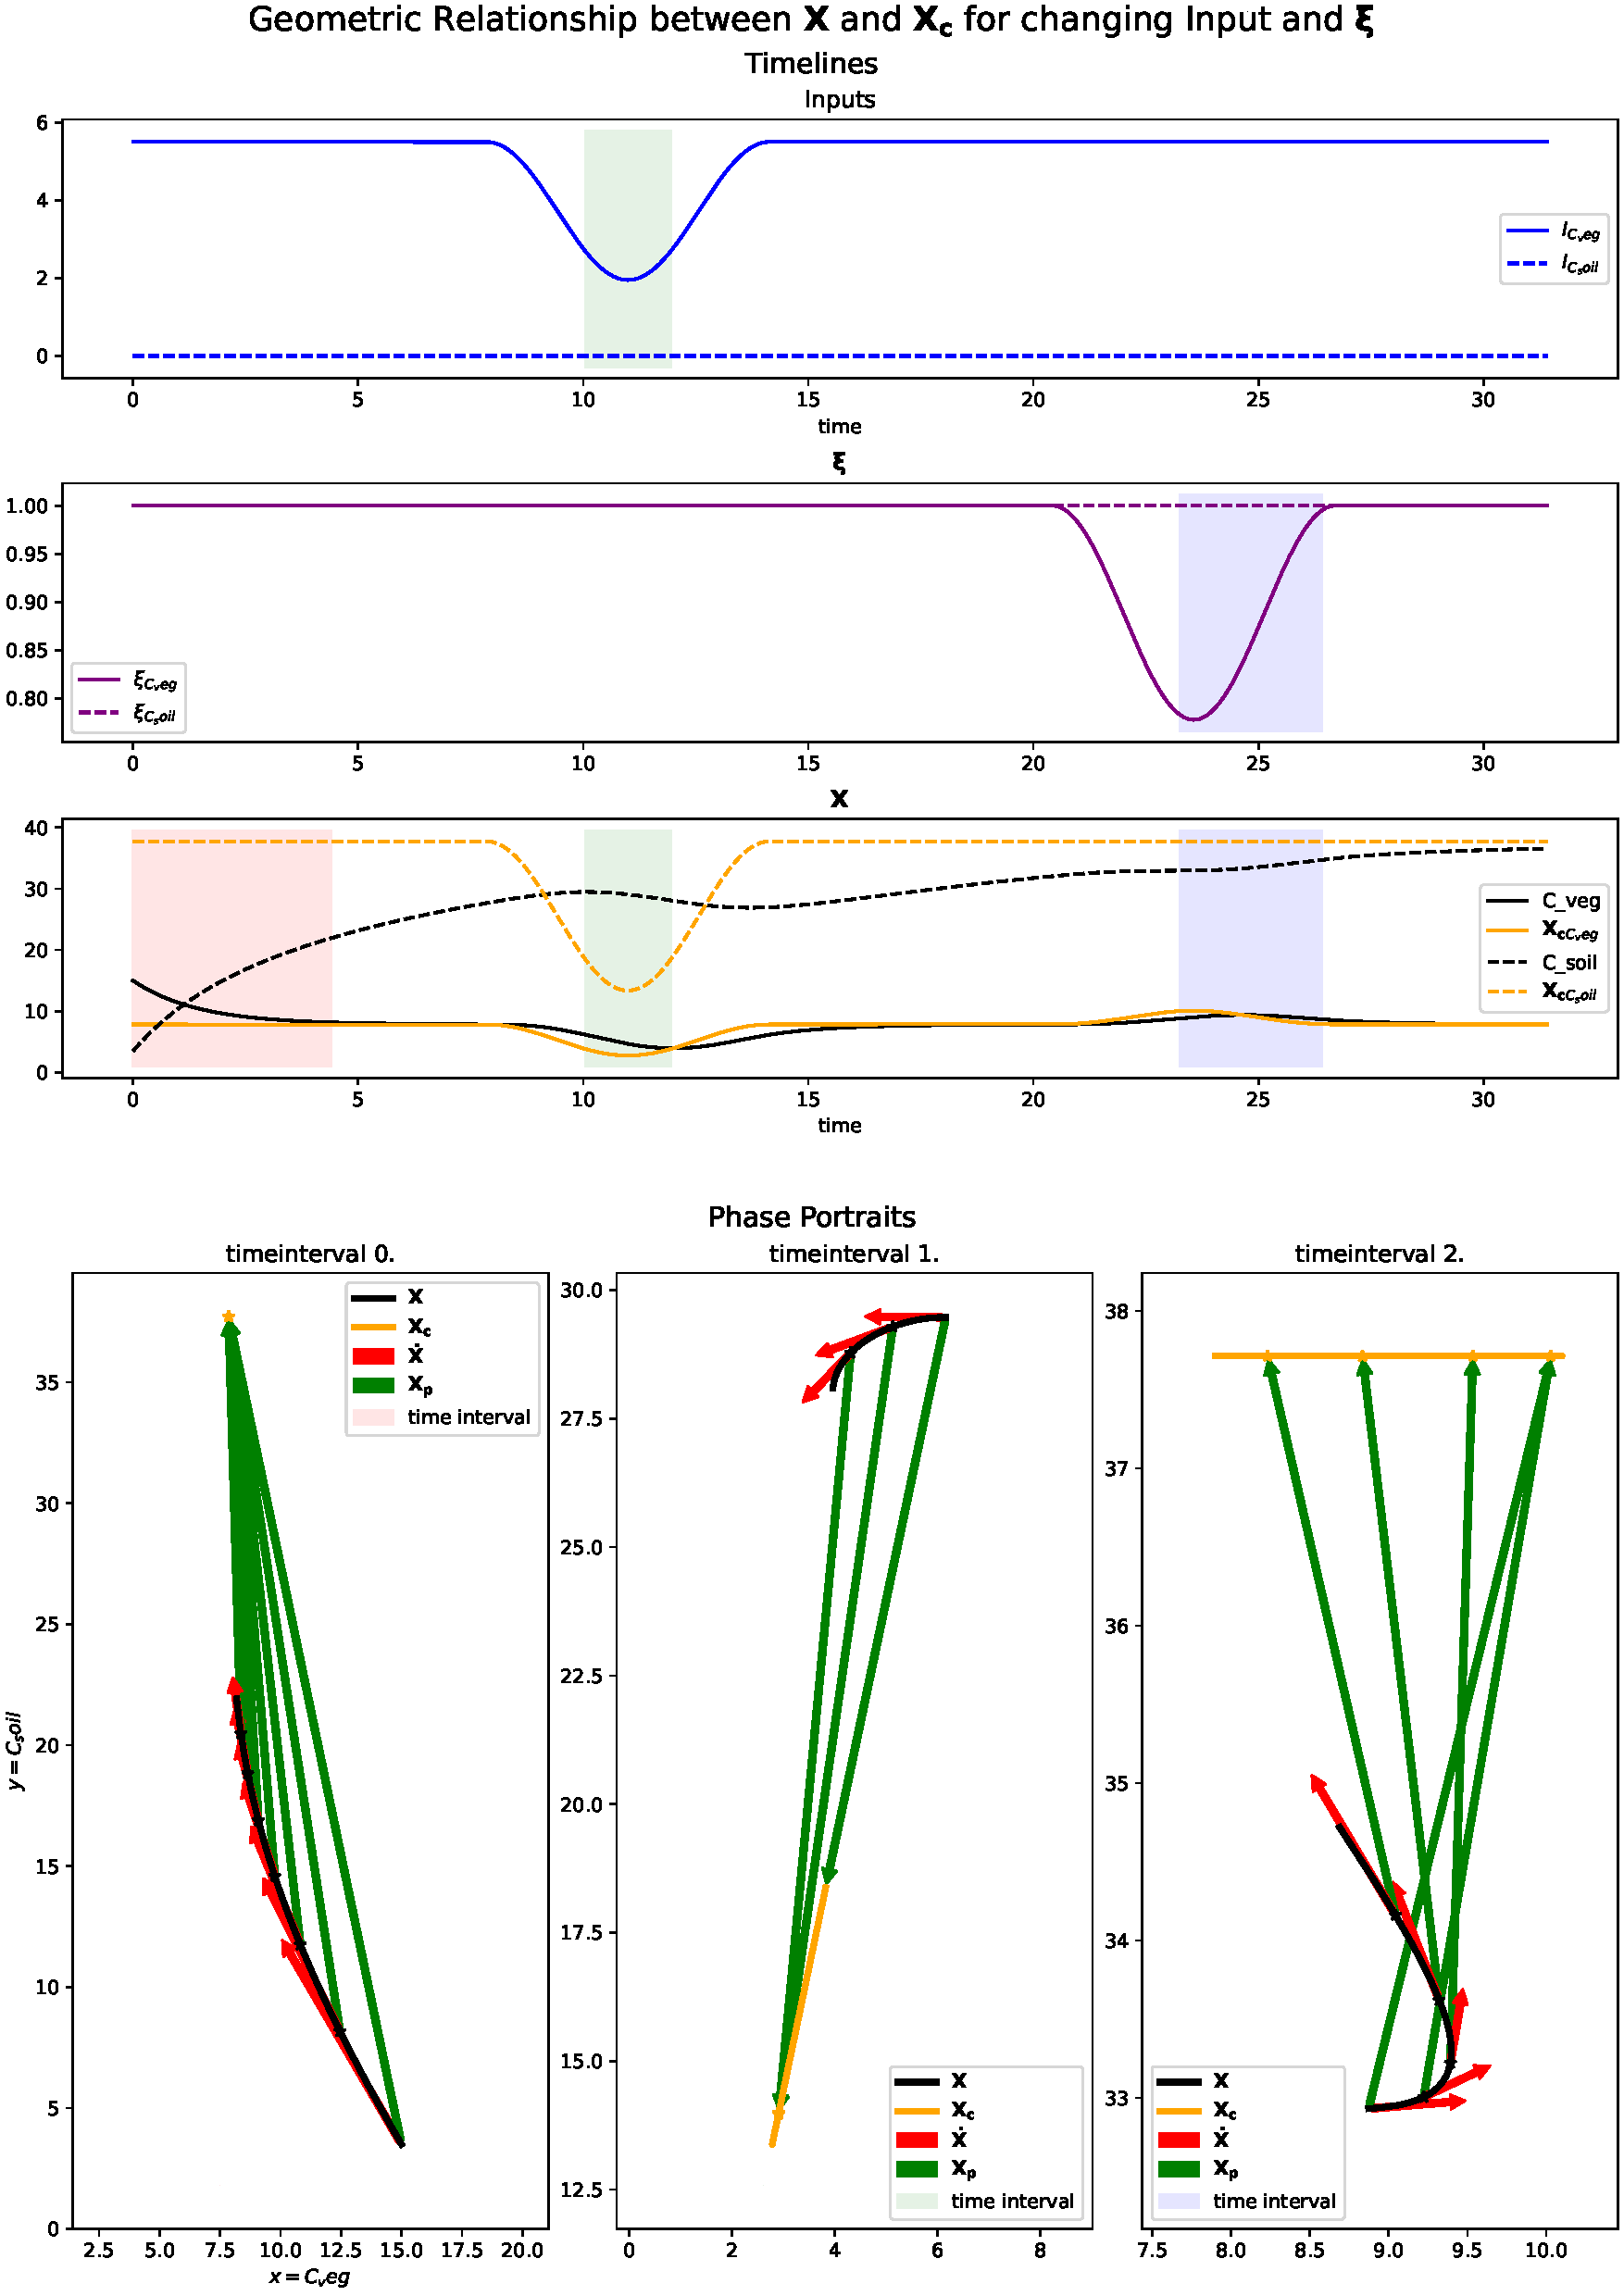
\includegraphics[height=.9\textheight]{figures/combined_timelines_and_2d_phase_space.pdf}
\caption{
  \label{Xc2D}
}
\end{figure}

\begin{figure}[t]
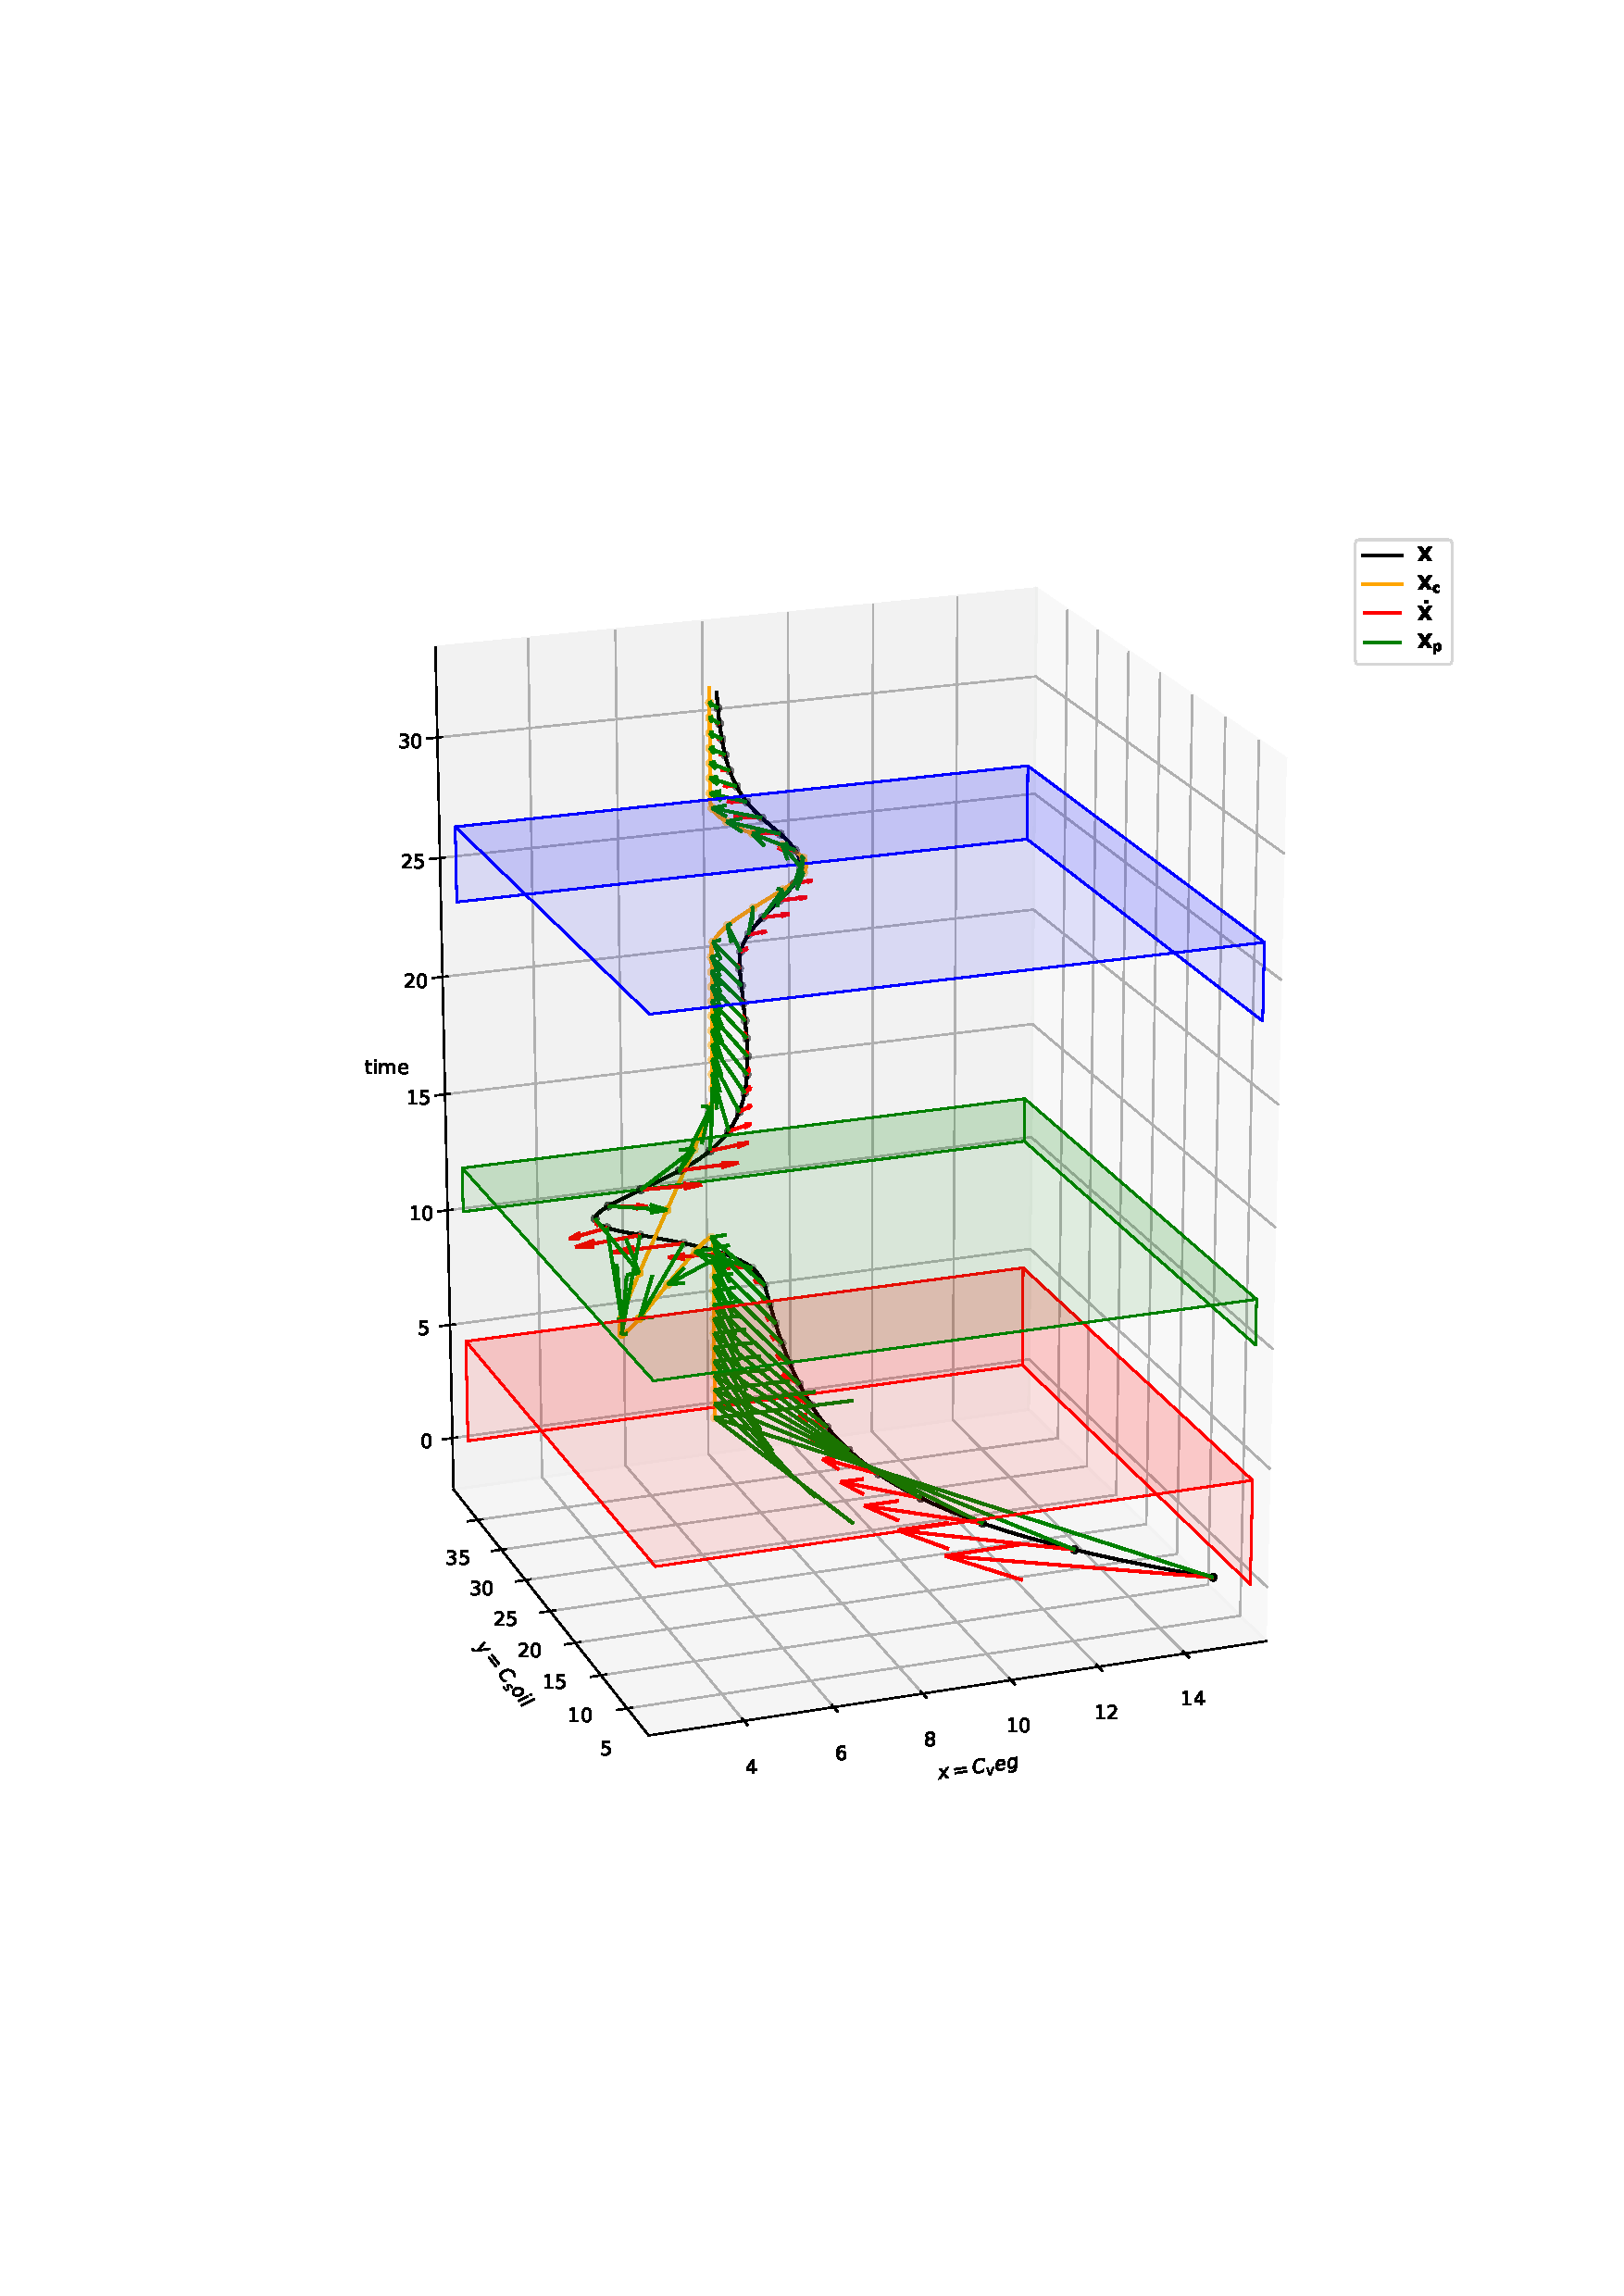
\includegraphics[height=.9\textheight]{figures/plot_vector_3d_X_Xc_time_z.pdf}
\caption{
  \label{Xc3D}
  %The 3D plot shows the same trajectories as \figref{}
  %For the first period
  %of its timeline (bottom) to $t\approx 2\pi$. In this period $X_c$ stays constant and
  %$X$ gradually approaches $X_c$ (although the derivative is not parallel to $X_p$).
  %after}
}
\end{figure}
\subsubsection{surrogate system for the overall mass}
We are aiming at something like this:
$$
\dot{x}=u(t)-m(t)x
$$ 
where $x$ is the aggregated mass over all pools.
The question is how to specify $m(t)$ to insure this.

We start with the special case of a linear but nonautonomous system (which is the subject of \citep{Luo2017Biogeosciences}):
$$
\frac{d \X}{d t}= \I(t) - M(t) \X 
$$
Taking the sum over all pools yields.
$$
\sum_{p \in pools} \left( \frac{d \X}{d t} \right)_p
=
\left( \I(t) - M(t) \X \right)_p
$$

With: 
$$
u=\sum_{p \in pools} (\I)_p, 
$$
$$
x = \sum_{p \in pools} (\X)_p
\text{ and }
$$ 
$$
\sum_{p \in pools} \left( \frac{d \X}{d t} \right)_p
=\frac{d}{d t}\sum_{p \in pools} (\X )_p
=\frac{d}{d t} x
$$
We can now try to construct our new system for the combined mass $x$, in particular we want to find a function for the time dependent rate $m(t)$ such that. 
$$
\dot{x}
=u(t)-m(t) x 
=\sum_{p \in pools} \left( \I(t) - M(t) \X \right)_p
=u(t)-\sum_{p \in pools} ( M(t) \X )_p
$$
This yields: 
$$
m(t) = \frac{
    \sum_{p \in pools} ( M(t) \X )_p
    }{
    \sum_{p \in pools} (\X)_p
    }
$$
Notes:
\begin{enumerate}
\item 
  $m$ will in general be a function of time $m(t)$ even if the original matrix $M$ is not.
  This becomes apparent when we consider that we need the vector $\X$ for every $t$ to define $m(t)$, which means that we also must solve the original system at least simultaneously.
  Assuming that we have done so \emph{before} we we can write a little more obviously.
  $$
  m(t) = \frac{
      \sum_{p \in pools} ( M \X(t) )_p
      }{
      \sum_{p \in pools} (\X(t))_p
      }
  $$
  Intuitively this reflects that the original system can have different rates for different pools and so the overall 
  rate depends on how mass is distributed between the pools initially and by the input streams. 
  The fact that the surrogate system is specific to a particular solution of the original system becomes even more apparent
  if we build surrogate systems for a nonlinear system. 
\item
  Consider a nonlinear systems
  $$
  \frac{d \X}{d t}= \I(\X,t) - M(\X,t) \X 
  $$
  Assume that we first solve the system numerically and therefore have $\X(t)$ available.
  Substituting the solution we get a linear system:
  $$
  \frac{d \X}{d t}= \tilde{\I}(t) - \tilde{M}(t) \X 
  $$
  with 
  $$
  \tilde{\I}(t)=\I(\X(t),t)
  $$
  and
  $$
  \tilde{M}(t)=M(\X(t),t)
  $$
  Which allows us to construct a one pool surrogate system with the same solution.
\end{enumerate}

The connection between the directions of $X_c$ and $X$ can be formalized in the following observations.

\begin{observation}[$x_p$ and $\dot{x}$ for the surrogate system]
With
\begin{align*}
\dot{x}   &=   u(t)-m(t)x              \\
x_c       &=   \frac{1}{m(t)} u(t)    \\
x_p       &=   x_c-x                  \\
          &=   \frac{1}{m(t)} \dot{x} 
\end{align*}
we have:
\begin{align}
\label{sign}
\sign \dot{x} &= \sign x_p
\end{align}
Which means that the solution $x$ always increases if $x<x_c$ and always decreases if $x>x_c$.
This is clear since $m(t) \ge 0 \quad \forall t$ (in compartmental systems only positive fluxes are allowed) and $m \ne 0$ for $x_p$ and $x_c=\frac{1}{m(t)} u$ to be defined.
\end{observation}

\begin{observation}[$\X_p$ and $\dot{\X}$ are not parallel]
An attempt to generalize \eqref{sign} to vectors in the sense that $\X_p$ and $\dot{\X}$ point in the same direction fails.
In \figref{Xc3D} the temporal evolution of $\X_c$ and $\X$ for an example two pool system is plotted,
which shows that in general $\X_p$ and $\dot{\X}$ are not pointing in the same direction.
\begin{align}
\frac{d}{dt}\left[\begin{matrix}C_{veg}\\C_{soil}\end{matrix}\right] = \left[\begin{matrix}I_{veg}{\left(t \right)}\\0\end{matrix}\right] + \left[\begin{matrix}- \left(r_{veg2out} + r_{veg2soil 0}\right) \xi_{veg}{\left(t \right)} & 0\\r_{veg2soil 0} \xi_{veg}{\left(t \right)} & - r_{soil2out}\end{matrix}\right] \left[\begin{matrix}C_{veg}\\C_{soil}\end{matrix}\right]
\end{align}
\begin{align}
\left[\begin{matrix}\frac{1}{\left(r_{veg2out} + r_{veg2soil 0}\right) \xi_{veg}{\left(t \right)}} & 0\\\frac{r_{veg2soil 0}}{r_{soil2out} \left(r_{veg2out} + r_{veg2soil 0}\right)} & \frac{1}{r_{soil2out}}\end{matrix}\right]
\end{align}
\begin{align}
\left[\begin{matrix}\frac{I_{veg}{\left(t \right)}}{\left(r_{veg2out} + r_{veg2soil 0}\right) \xi_{veg}{\left(t \right)}}\\\frac{r_{veg2soil 0} I_{veg}{\left(t \right)}}{r_{soil2out} \left(r_{veg2out} + r_{veg2soil 0}\right)}\end{matrix}\right]
\end{align}
This is even the case if we only consider autonomous systems.
Although $\X_c$ IS the unique stable fixpoint (and therefore an attractor) for $\tilde{\X}$ the  solution of the autonomous system, even $\dot{\tilde{\X}}$ does in general NOT point in the direction of $\X_c-\tilde{\X}$. This is a reflection of the internal pool structure as represented in  $M$. Compartmental systems are in general not obliged to move straight through phase space.   
%E.g. a serial system of three pools can only get material from pool 1 to pool 3 via pool 2. This might dictate a curved path to the equilibrium value, temporarily increasing the content of the
%intermediate pool.
\end{observation}

\begin{observation}[Direction of $\X_p$ and $\dot{\X}$]
A minimal attempt to generalize \eqref{sign} is the following:
If $M(t)$ is invertable 
% (this excludes zero rates) 
and if all components of the derivative $\dot{\X}$ have the same sign then all components of the $\X_p=\X_c-\X$ have the same sign too.
In other words if $\dot{\X}$ occupies the non negative orthant so does $\X_p$ and if $\dot{\X}$ occupies the non positive orphant so does $\X_p$. In both cases the scalar product $\langle \dot{\X},\X_p \rangle \ge 0$

Proof:
Using that $M(t)$ is invertable we can write the steady state solution $\X^*$ (for the system frozen at time $t$) for a given constant input $\I$ and Matrix $M$ as
\begin{align}
\X^*=M^{-1}\I
\end{align}
We first convince ourselves that the matrix $M^{-1}$ has indeed only positive elements.
For a compartmental system the pool contents and inputs are always positive.
This is also true for the steady state values of the frozen system.
If we choose $\I = (1,0,\dots, 0) $ we get $\X^*=M_{:,1}$ so we know that 
the first column of $M$ must be positive. 
We can do this with any column to obtain $M_{i,j}>0 \quad \forall i,j$.
If we assume further that the derivative $\dot{\X}$ has only positive components then the components of 
$\X_p$ are sums of products of positive values and have to be positive too.
In case all the components of $\dot{\X}$ are negative then the components of $\X_p$ are negative by the same argument.
A consequence of this statement is that in case $\dot{\X}$ is either completely in the positive or negative orthant the inner product $\langle \dot{\X},\X_p \rangle \ge 0$ which means that the angle between them is smaller than a right angle.

Unfortunately this argument only applies to the very special cases that all pools increase or decrease simultaneously.
In general $\dot{\X}$ as well as $\X_p$ can have positive and negative components but in this case the knowledge of the positive
of $M^{-1}$ is not sufficient to confine the difference in their directions.
\end{observation}

\begin{observation}[Direction of $\X_p$ and $\dot{X}$ in special cases]
The previous observation leads to the conjecture that perhaps $\langle \dot{\X},\X_p \rangle \ge 0$ is generally true, even if $M_{i,j} > 0 $ is not sufficient to prove it.
There are however special cases where this can be ascertained.
If we talk about $\X_c$ at all we assume the existence of a stable fixed point for the frozen system. A necessary (and sufficient) condition for this is that the real parts of all the eigenvalues of $M$ are greater than zero. 
In case all the eigenvalues are real we can express $\X_p$ and $\dot{\X}$ and the linear mapping encoded by $M$ in terms of tbe eigenvectors $e_1,\dots e_n$ and eigenvalues $\lambda_1, \dots \lambda_n$.
\begin{align}
\langle \dot{\X},\X_p  \rangle 
&=
\langle M \X_p,\X_p  \rangle \\
&=
\langle 
  \lambda_1 e_1 {x_p}_1+\dots \lambda_n e_n {x_p}_n , 
  e_1 {x_p}_1+\dots e_n {x_p}_n
\rangle 
\\
&=
\lambda_1 {x_p}_1^2 \langle e_1,e_1 \rangle
+\dots +
\lambda_n{x_p}_n^2 \langle e_n,e_n \rangle
\\
&> 0.
\end{align}
A noteworthy application are two dimensional compartmental linear systems with constant $M$ which can not have complex eigenvalues (Since the complex eigenvalues of real matrices always come in conjugate pairs the matrix of a two dimensional system would describe a rotation with shrinking radius (negative real part). For $\X$ on one of the boundaries of the positive orthant this would lead to a derivative pointing outwards and thus to negative pool contents, violating the assumption of a compartmental system).
If the system has more than two dimensions complex eigenvalues become possible and the discussion more complicated.
\end{observation}


\conclusions  %% \conclusions[modified heading if necessary]
TEXT
{\color{red} summary still missing}

\begin{enumerate}
\item
$X_c$ is not an attractor for $\X$ neither is $x_c$ for $x$ (overall mass)
All derived variables like $\RT$ and $\tau$ have to be interpreted in the context of the 'frozen' systems \emph{in equilibrium}.
\item
$\bar{X_c}$ as proxy for $\X$ depends on the time interval (examples show minimal error of about 7/100)
\item
$\xi$ is not a model property but a property of the literature
In attributions it is saver to look at $k \xi$ 


\end{enumerate}

%% The following commands are for the statements about the availability of data sets and/or software code corresponding to the manuscript.
%% It is strongly recommended to make use of these sections in case data sets and/or software code have been part of your research the article is based on.

\codeavailability{TEXT} %% use this section when having only software code available


\dataavailability{TEXT} %% use this section when having only data sets available


\codedataavailability{TEXT} %% use this section when having data sets and software code available


\sampleavailability{TEXT} %% use this section when having geoscientific samples available


\videosupplement{TEXT} %% use this section when having video supplements available


%%%%%%%%%%%%%%%%%%%%%%%%%%%%%%%%%%%%%%%%%%%%%%%%%%%%%%%%%%%%%%%%%%%%%%%%%%%%%%%%%%%%%%%%%%%%%%%%%%%%%%%%%%%%%%%%%%%%
%%%%%%%%%%%%%%%%%%%%%%%%%%%%%%%%%%%%%%%%%%%%%%%%%%%%%%%%%%%%%%%%%%%%%%%%%%%%%%%%%%%%%%%%%%%%%%%%%%%%%%%%%%%%%%%%%%%%
\appendix
\section{$\xi$}    %% Appendix A

\subsection{Examples where the actual value of $\xi$ matters or does not matter}     %% Appendix A1, A2, etc.
\label{xi_examples}
E.g. consider variance attribution via covariance as described in the supplementary material S(9) of \citep{Zhou2018JOC}.
The relative contribution $RVar(a b)_a$ of variable $a$ to the variance of the product $a b$ is defined as 
\begin{align}
  \label{covln}
  RVar(a b)_a = \frac{cov(ln(a),ln(a b)}{Var(ln(a b)} 
\end{align}
As an example for an attribution that is independent of the arbitrary $d$
consider the question of temporal variance of $rt$ to it's factors $\xi$ and
$br$ via (temporal) covariance of $rt$ with $\xi$ and $k$ since the temporal
covariance $ cov(ln(k),ln(rt))=0 $ but it is also obvious that an attribution to
the temporal change of $\xi$ leads to the same result as an attribution to the
product $\xi k$, so the distinction between contributions of $\xi$ and $k$ is
not necessary.  
% {\color{blue} perhaps cite \citep{Jiang2017James} if I find the
% place where the attribution is described. Actually the total difference in
% $\xi(t_{end})-\xi(t_0)$ is discussed which \emph{would} change with a scaled $\xi$
% but this does not seem to matter in the paper (since it is the same model and
% the \emph{same} $k$ and $\xi$ are used } 
An example where the result does
depend on the arbitrary $d$ is given by the attribution of the variance of $\RT$
of model ensemble to the variance of $\xi$ and $k$ via the same method as the
following minimal ensemble of two models shows. If we look at the contribution
of $\xi$ to the variance
\begin{align}
{var_{\xi}}_{rel} = \frac{
  cov([ln(\xi_1),ln(\xi_2)]^T,[ln(\frac{k_1}{\xi_1}),ln(\frac{k_2}{\xi_2})]^T)
}{
  var([ln(\frac{k_1}{\xi_1}),ln(\frac{k_2}{\xi_2})]^T)
}
\end{align}
If we rewrite the second model in the vector with an arbitrary $d$ we get a different result



\noappendix       %% use this to mark the end of the appendix section. Otherwise the figures might be numbered incorrectly (e.g. 10 instead of 1).

%% Regarding figures and tables in appendices, the following two options are possible depending on your general handling of figures and tables in the manuscript environment:

%% Option 1: If you sorted all figures and tables into the sections of the text, please also sort the appendix figures and appendix tables into the respective appendix sections.
%% They will be correctly named automatically.

%% Option 2: If you put all figures after the reference list, please insert appendix tables and figures after the normal tables and figures.
%% To rename them correctly to A1, A2, etc., please add the following commands in front of them:

\appendixfigures  %% needs to be added in front of appendix figures

\appendixtables   %% needs to be added in front of appendix tables

%% Please add \clearpage between each table and/or figure. Further guidelines on figures and tables can be found below.



\authorcontribution{TEXT} %% this section is mandatory

\competinginterests{TEXT} %% this section is mandatory even if you declare that no competing interests are present

\disclaimer{TEXT} %% optional section

\begin{acknowledgements}
TEXT
\end{acknowledgements}




%% REFERENCES

%% The reference list is compiled as follows:

%%\begin{thebibliography}{}
%%
%%\bibitem[AUTHOR(YEAR)]{LABEL1}
%%REFERENCE 1
%%
%%\bibitem[AUTHOR(YEAR)]{LABEL2}
%%REFERENCE 2
%%
%%\end{thebibliography}

%% Since the Copernicus LaTeX package includes the BibTeX style file copernicus.bst,
%% authors experienced with BibTeX only have to include the following two lines:
%%
%% \bibliographystyle{copernicus}
%% \bibliography{example.bib}
%%
%% URLs and DOIs can be entered in your BibTeX file as:
%%
%% URL = {http://www.xyz.org/~jones/idx_g.htm}
%% DOI = {10.5194/xyz}


%% LITERATURE CITATIONS
%%
%% command                        & example result
%% \citet{jones90}|               & Jones et al. (1990)
%% \citep{jones90}|               & (Jones et al., 1990)
%% \citep{jones90,jones93}|       & (Jones et al., 1990, 1993)
%% \citep[p.~32]{jones90}|        & (Jones et al., 1990, p.~32)
%% \citep[e.g.,][]{jones90}|      & (e.g., Jones et al., 1990)
%% \citep[e.g.,][p.~32]{jones90}| & (e.g., Jones et al., 1990, p.~32)
%% \citeauthor{jones90}|          & Jones et al.
%% \citeyear{jones90}|            & 1990

\bibliographystyle{copernicus}
\bibliography{TEE-clean.bib}


%% FIGURES

%% When figures and tables are placed at the end of the MS (article in one-column style), please add \clearpage
%% between bibliography and first table and/or figure as well as between each table and/or figure.

% The figure files should be labelled correctly with Arabic numerals (e.g. fig01.jpg, fig02.png).


%% ONE-COLUMN FIGURES

%%f
%\begin{figure}[t]
%\includegraphics[width=8.3cm]{FILE NAME}
%\caption{TEXT}
%\end{figure}
%
%%% TWO-COLUMN FIGURES
%
%%f
%\begin{figure*}[t]
%\includegraphics[width=12cm]{FILE NAME}
%\caption{TEXT}
%\end{figure*}
%
%
%%% TABLES
%%%
%%% The different columns must be seperated with a & command and should
%%% end with \\ to identify the column brake.
%
%%% ONE-COLUMN TABLE
%
%%t
%\begin{table}[t]
%\caption{TEXT}
%\begin{tabular}{column = lcr}
%\tophline
%
%\middlehline
%
%\bottomhline
%\end{tabular}
%\belowtable{} % Table Footnotes
%\end{table}
%
%%% TWO-COLUMN TABLE
%
%%t
%\begin{table*}[t]
%\caption{TEXT}
%\begin{tabular}{column = lcr}
%\tophline
%
%\middlehline
%
%\bottomhline
%\end{tabular}
%\belowtable{} % Table Footnotes
%\end{table*}
%
%%% LANDSCAPE TABLE
%
%%t
%\begin{sidewaystable*}[t]
%\caption{TEXT}
%\begin{tabular}{column = lcr}
%\tophline
%
%\middlehline
%
%\bottomhline
%\end{tabular}
%\belowtable{} % Table Footnotes
%\end{sidewaystable*}
%
%
%%% MATHEMATICAL EXPRESSIONS
%
%%% All papers typeset by Copernicus Publications follow the math typesetting regulations
%%% given by the IUPAC Green Book (IUPAC: Quantities, Units and Symbols in Physical Chemistry,
%%% 2nd Edn., Blackwell Science, available at: http://old.iupac.org/publications/books/gbook/green_book_2ed.pdf, 1993).
%%%
%%% Physical quantities/variables are typeset in italic font (t for time, T for Temperature)
%%% Indices which are not defined are typeset in italic font (x, y, z, a, b, c)
%%% Items/objects which are defined are typeset in roman font (Car A, Car B)
%%% Descriptions/specifications which are defined by itself are typeset in roman font (abs, rel, ref, tot, net, ice)
%%% Abbreviations from 2 letters are typeset in roman font (RH, LAI)
%%% Vectors are identified in bold italic font using \vec{x}
%%% Matrices are identified in bold roman font
%%% Multiplication signs are typeset using the LaTeX commands \times (for vector products, grids, and exponential notations) or \cdot
%%% The character * should not be applied as mutliplication sign
%
%
%%% EQUATIONS
%
%%% Single-row equation
%
%\begin{equation}
%
%\end{equation}
%
%%% Multiline equation
%
%\begin{align}
%& 3 + 5 = 8\\
%& 3 + 5 = 8\\
%& 3 + 5 = 8
%\end{align}
%
%
%%% MATRICES
%
%\begin{matrix}
%x & y & z\\
%x & y & z\\
%x & y & z\\
%\end{matrix}
%
%
%%% ALGORITHM
%
%\begin{algorithm}
%\caption{...}
%\label{a1}
%\begin{algorithmic}
%...
%\end{algorithmic}
%\end{algorithm}
%
%
%%% CHEMICAL FORMULAS AND REACTIONS
%
%%% For formulas embedded in the text, please use \chem{}
%
%%% The reaction environment creates labels including the letter R, i.e. (R1), (R2), etc.
%
%\begin{reaction}
%%% \rightarrow should be used for normal (one-way) chemical reactions
%%% \rightleftharpoons should be used for equilibria
%%% \leftrightarrow should be used for resonance structures
%\end{reaction}
%
%
%%% PHYSICAL UNITS
%%%
%%% Please use \unit{} and apply the exponential notation
%%%%%%%%%%%%%%%%%%%%%%%%%%%%%%%%%%%%%%%%%%%%%%%%%%%%%%%%%%%%%%%%%%%%%%%%%%%%%%%%%%%%%%%%%%%%%%%%%%%%%%%%%%%%%%%%%%%%
%%%%%%%%%%%%%%%%%%%%%%%%%%%%%%%%%%%%%%%%%%%%%%%%%%%%%%%%%%%%%%%%%%%%%%%%%%%%%%%%%%%%%%%%%%%%%%%%%%%%%%%%%%%%%%%%%%%%
\section{to do}
\begin{enumerate}
\item
  finish the figure
\item
  \sout{introduce the 1D surrogate systems}
\item
  \sout{Prove the geometric Observations} 
\item
  Put the definition for attractors in the text
\item 
To explain the 1 pools system tendency to "chase" $X_c$ we can rephrase it the other way around to:
At a given point $t_f$the derivative is determined by the present $m_f=m(t_f)$ 
and the present input $i_f=i(t_f)$:$\dot{x} = i_f-m_f x_f$ 
The derivative at this point determines the possible equilibrium of the frozen linear system with the same derivative at this point.
If the derivative is positive we have 
\begin{align*}
0 < if - m_f x \\
\rightarrow 
m_f x & < i_f \\
\rightarrow 
x < \frac{1}{m_f} i_f=x_f* = x_c
\end{align*}
So the prospective equilibrium of the frozen system is bigger than the current value.
\end{enumerate}
\end{document}
